\subsection{ML Revised Evaluation}
Three evaluation assumptions in the original ML pipeline inflate the reported ADR from $\approx\svmADR$ to near-perfect $\svmOrigADR$ when all corrections are removed
(Fig.~\ref{fig:bias_progression}). The corrected SVM (Fix~1+2+3 with balanced class weights) forms the revised ML baseline for all subsequent comparisons. Full methodology and per-revision breakdown are given in Appendix.

\begin{figure}[htbp]
  \centering
  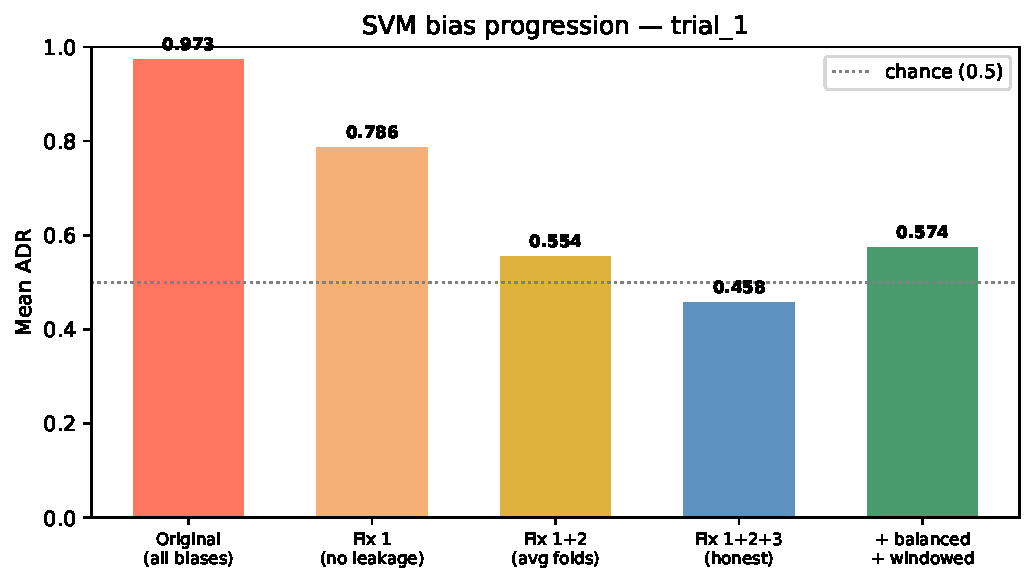
\includegraphics[width=\columnwidth]{figures/fig_bias_progression}
  \caption{SVM ADR across pipeline variants (trial\_1). Each correction removes one source of optimistic assumption; the rightmost bar is the revised baseline.}
  \label{fig:bias_progression}
\end{figure}

\subsection{Initial DL Evaluation (5 Seeds)}

Table~\ref{tab:dl_results} reports ADR for each DL model under a group-aware
70/15/15 split, averaged over five random seeds (trial\_1). All three models
achieve ADR between 0.62 and 0.68.

\begin{table}[htbp]
\centering
\caption{DL model ADR on held-out test set (trial\_1, 5 seeds).}
\label{tab:dl_results}
\begin{tabular}{lc}
\toprule
\textbf{Model} & \textbf{ADR (mean $\pm$ std)} \\
\midrule
MLP-FV            & \mlpADR \\
GRU-DGT           & \gruADR \\
BiGRU+TF-Aug & \bigruADR \\
\bottomrule
\end{tabular}
\end{table}

\begin{figure}[htbp]
  \centering
  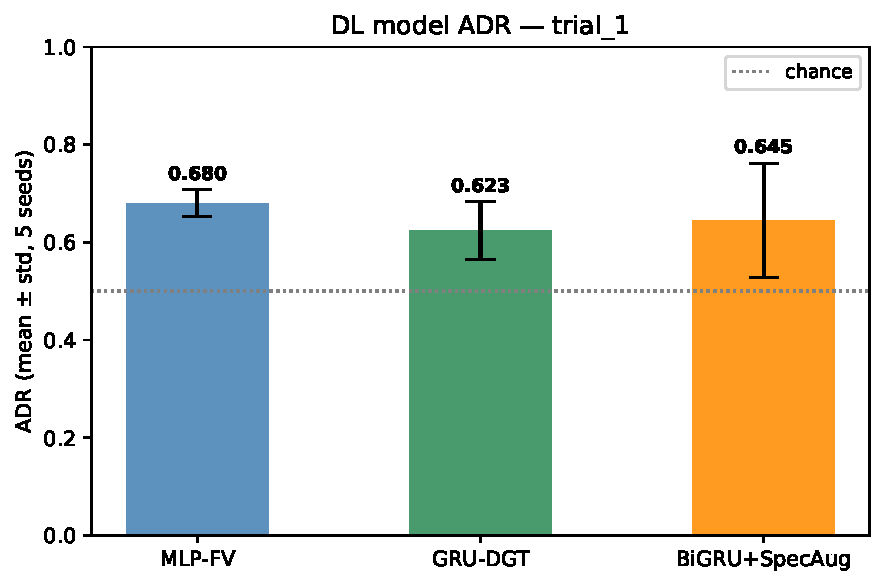
\includegraphics[width=\columnwidth]{figures/fig_dl_adr}
  \caption{DL model ADR (mean $\pm$ std, 5 seeds, trial\_1). The wide error bar on BiGRU signals that five seeds are insufficient for reliable conclusions.}
  \label{fig:dl_adr}
\end{figure}

The BiGRU in particular exhibits high variance (seed ADR range \bigruSeedADRMin--\bigruSeedADRMax). With only
$n=5$ seeds the confidence intervals are too wide to draw reliable conclusions
about relative model performance. This motivated adopting LOTO cross-validation as the primary evaluation protocol, maximising use of the limited dataset.

\subsection{LOTO Cross-Validation (Primary Evaluation)}

LOTO (Leave-One-Transient-Out) holds out one complete transient per fold, making use of every available sample while remaining strictly transient-aware. Table~\ref{tab:loto} reports per-device ADR and EER for the BiGRU on trial\_1. Mean ADR is \bigruLOTOadrMean{} and mean EER is \bigruLOTOeerMean{}, well above the chance EER of 0.5, confirming above-chance device discrimination across all authorized devices.

\begin{table}[htbp]
\centering
\caption{BiGRU LOTO per-device ADR and EER (trial\_1).}
\label{tab:loto}
\begin{tabular}{lcc}
\toprule
\textbf{Device} & \textbf{ADR} & \textbf{EER} \\
\midrule
device2  & \bigruLOTOadrTwo   & \lotoEERTwo \\
device3  & \bigruLOTOadrThree & \lotoEERThree \\
device9  & \bigruLOTOadrNine  & \lotoEERNine \\
device12 & \bigruLOTOadrTwelve & \lotoEERTwelve \\
\midrule
\textbf{Mean} & \textbf{\bigruLOTOadrMean} & \textbf{\bigruLOTOeerMean} \\
\bottomrule
\end{tabular}
\end{table}

\begin{figure}[htbp]
  \centering
  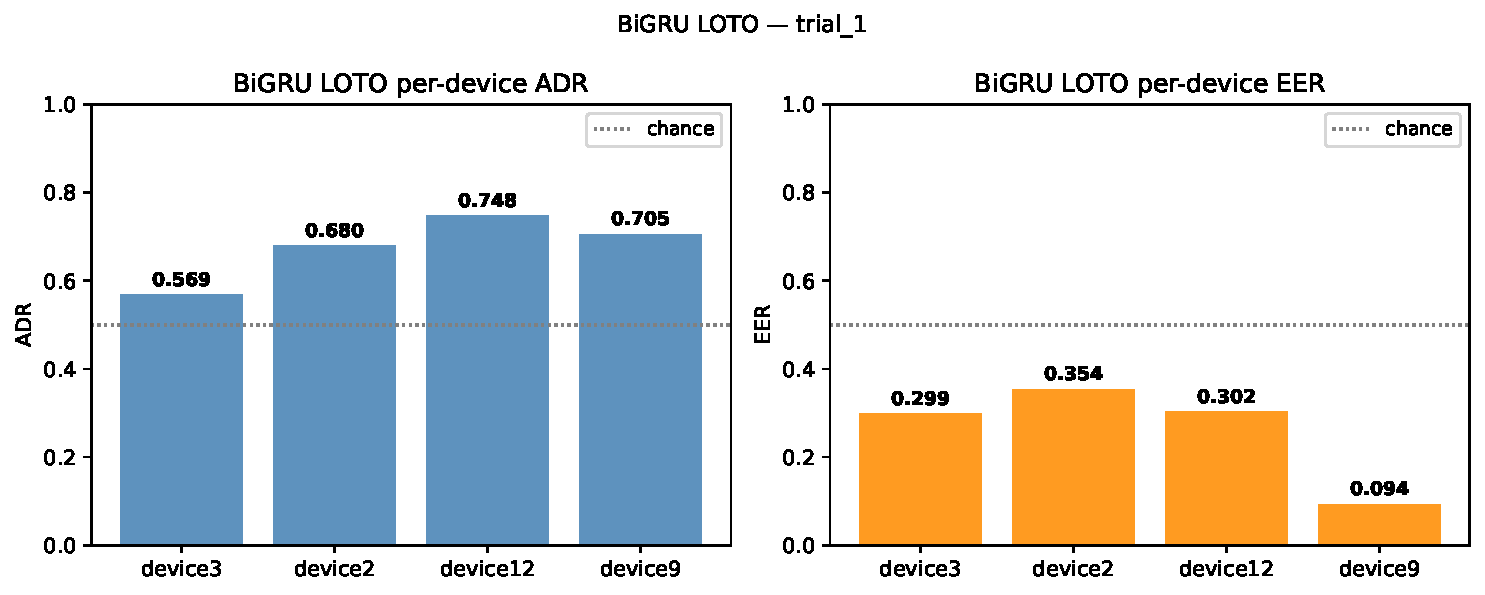
\includegraphics[width=\columnwidth]{figures/fig_loto_eer}
  \caption{BiGRU LOTO per-device ADR and EER (trial\_1). Dashed line marks chance level (EER~$= 0.5$).}
  \label{fig:loto_eer}
\end{figure}

\subsection{ML vs.\ DL Comparison}

Fig.~\ref{fig:ml_vs_dl_loto} places the revised SVM alongside all three DL models
evaluated under LOTO cross-validation. No pipeline has a clear advantage: all models
cluster in a \svmADR--\bigruLOTOadrMean{} ADR band with overlapping uncertainty. The performance gap
between the original and revised pipelines is entirely attributable to evaluation
methodology.

\begin{figure}[htbp]
  \centering
  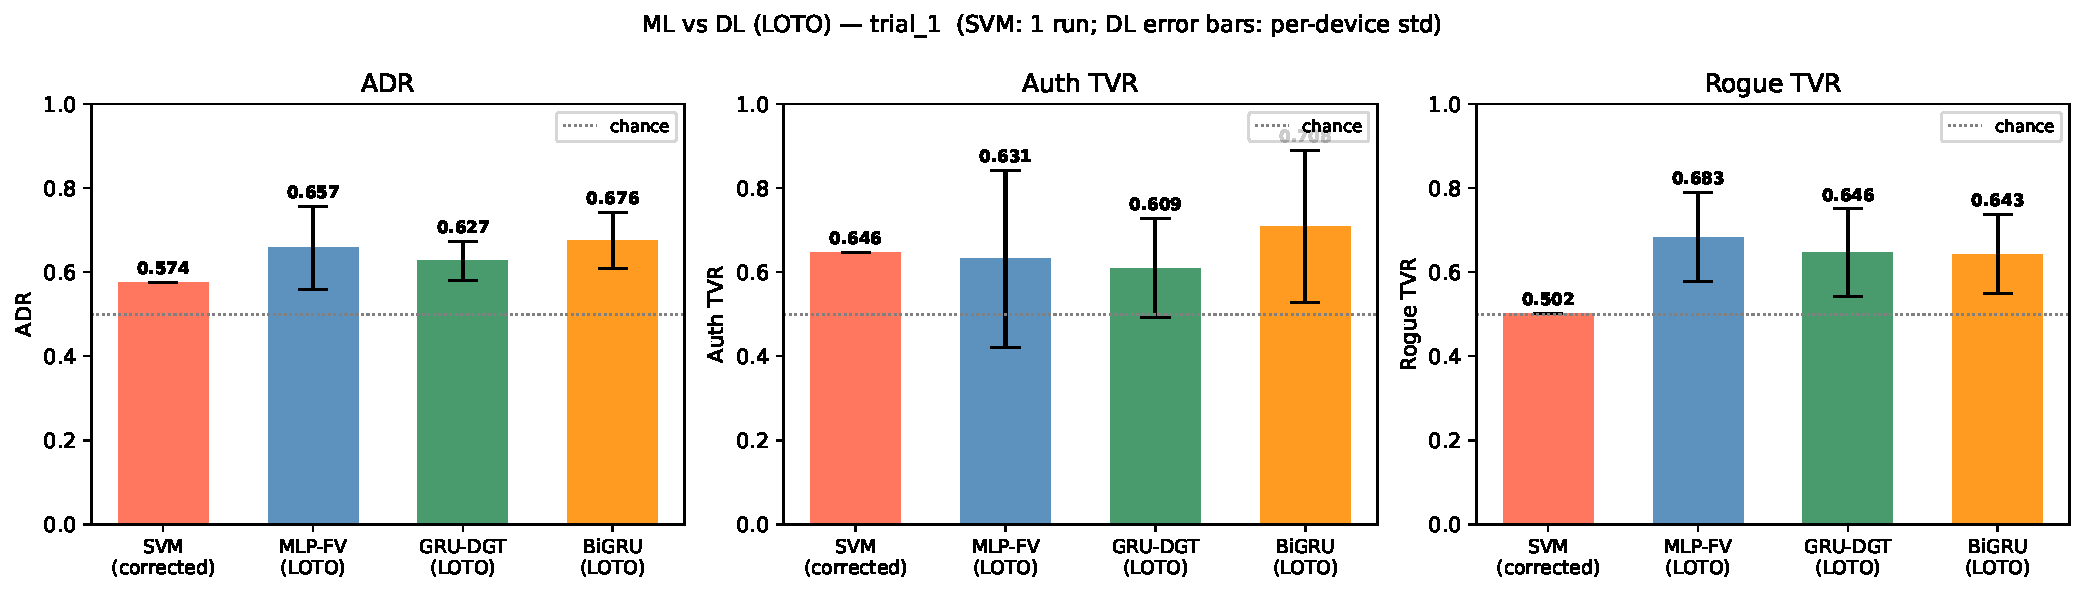
\includegraphics[width=\columnwidth]{figures/fig_ml_vs_dl_loto}
  \caption{ML vs.\ DL (LOTO): ADR, Auth TVR, and Rogue TVR (trial\_1).
           SVM error bar is zero (single deterministic run);
           DL bars are $\pm$1 std across authorized devices (LOTO).}
  \label{fig:ml_vs_dl_loto}
\end{figure}
